%  Typ dokumentu - článek, prezentace aj.
\documentclass[english]{article}

%  Nastaví vstupní a výstupní kódování znaků (encoding) a lokalizace
\usepackage[T1]{fontenc}
\usepackage[utf8]{inputenc}
\usepackage[english,czech]{babel}
\usepackage{icomma}

%  Formát papíru a odsazení od jeho okrajů
\usepackage[letterpaper]{geometry}
\geometry{verbose,tmargin=1.5cm,bmargin=2cm,lmargin=2cm,rmargin=2cm}

%  Umožňuje pracovat s grafikou
\usepackage{graphicx}
\usepackage{bigstrut}

%  Automaticky odsadí i první paragraf v každé sekci
\usepackage{indentfirst}

%  Umožňuje rozdělovat obsah na více sloupců
\usepackage{multicol}
\usepackage{booktabs}

%  Umožňuje používat hypertextové odkazy, nastavuje jejich barvu a
%  vlastnosti
\usepackage[unicode]{hyperref}
\hypersetup{
colorlinks=true, citecolor=blue, filecolor=blue, linkcolor=blue,
urlcolor=blue
}

%  Umožnění odstranění italiky u jednotek
\newcommand{\unit}[1]{\mathrm{#1}}

%  Formátování stránek, empty = odstraní číslování
% \pagestyle{empty}

%  Řádkování
\linespread{1.2}

%  Lepší zobrazování matematiky (rozšíření sum o \limits atd.)
\everymath{\displaystyle}
\usepackage{amsmath, amsthm, amssymb}

% Umožní psát přes \mathbb{N/R/Q/..} množiny čísel
\usepackage{amssymb}

%  Velikost fontu matematických výrazů v dokumentu lze pro danou
% základního fontu dokumentu upravit pomocí:
% \DeclareMathSizes{X}{Y}{Z}{U} kde:
% X je velikost fontu v dokumentu, pro kterou se matematika upraví
% Y je standartní velikost fontu matematiky
% Z je velikost fontu zmenšených (vnořených výrazů)
% U je velikost fontu ještě více zmenšených (vnořených výrazů).
\DeclareMathSizes{10}{10.5}{9}{9}

%  Nastaví autora, název, datum, skupinu měření apod. (můj vlastní
% příkaz, umožní znovu-použití v dokumentu)
\newcommand{\Author}{David Roesel}
\newcommand{\Coauthor}{Tereza Schönfeldová}
\newcommand{\Institute}{FJFI ČVUT v Praze}
\newcommand{\Subject}{FYZIKÁLNÍ PRAKTIKUM II}
\newcommand{\Group}{7}
\newcommand{\Circle}{ZS 7}
\newcommand{\Title}{Úloha \#7  \\Měření spektra gama záření scintilačním počítačem}
\newcommand{\Date}{24.2.2014}

% Začátek dokumentu - Formátování na výstup
\begin{document}

% Interní proměnné, možno zobrazovat u prezentací, používají se při
% generování pomocí \titlepage apod.
\author{\Author}
\title{\Title}
\date{\Date}

%  Lokalizace některých názvů do češtiny
\renewcommand{\figurename}{Obr.}
\renewcommand{\tablename}{Tab.}
\renewcommand{\refname}{Reference}

% --- Hlavička dokumentu -----------------------------------------------

\setlength{\parindent}{0cm}
\begin{multicols}{2}
\textbf{\Subject \\
        \Institute \\[0.1cm]
%\large  \Title \\[0.5cm]
\Title \\[0.5cm]
}
\begin{tabular}{rlrl}
\large Datum měření: & \Date & \large Skupina: & \Group \\
\large Jméno: & \Author & \large Kroužek:  & \Circle\\
\large Spolupracovala: & \Coauthor &\large Klasifikace:\\
\end{tabular}

\begin{flushright}

\includegraphics[scale=0.28]{../../_meta/fjfi_standart.pdf}
\hspace{0.2cm}

\includegraphics[scale=0.28]{../../_meta/cvut_standart.pdf}
\end{flushright}
\end{multicols}
\hrule
\vspace{0.5cm}

% ----------------------------------------------------------------------


% --- Tělo dokumentu ---------------------------------------------------
\setlength{\parindent}{0.5cm}
\section{Pracovní úkoly}

	\begin{enumerate}
		\item Osciloskopem pozorujte spektrum $^{137}$Cs na výstupu z jednokanálového analyzátoru. Načrtněte tvar spektra (závislost intenzity na energii záření) a přiložte k protokolu. (Osciloskop ukazuje tvary a amplitudy jednotlivých pulzů. Počet pulzů je dán intenzitou čáry a energie výškou impulzu.)
		\item Naměřte spektrum impulzů $^{137}$Cs jednokanálovým analyzátorem pomocí manuálního měření. Okno volte o šířce 100 mV. Spektrum graficky zpracujte. 
		\item Mnohokanálovým analyzátorem naměřte jednotlivá spektra přiložených zářičů ($^{137}$Cs, $^{60}$Co, $^{241}$Am a $^{133}$Ba). Určete výrazné píky a porovnejte je s tabulkovými hodnotami. (Každé spektrum nabírejte 10 minut.)
		\item Pomocí zářičů $^{137}$Cs a $^{60}$Co určete kalibrační křivku spektrometru a použijte ji při zpracování všech spekter naměřených mnohokanálovým analyzátorem. (Spektrum nabírejte 10 minut, použijte oba zářiče současně.)
		\item S využitím všech naměřených spekter určete závislost rozlišení spektrometru na energii gama záření. 
		\item Z naměřeného spektra $^{137}$Cs určete hodnotu píku zpětného rozptylu, Comptonovy hrany, energii rentgenového píku a energii součtového píku.
		\item Mnohokanálovým analyzátorem naměřte spektrum neznámého zářiče. Určete tento zářič, pozorujte a zaznamenejte další jevy v jeho spektru. (Spektrum nabírejte 10 minut.)
		\item Mnohokanálovým anlyzátorem naměřte spektrum pozadí v místnosti (zářiče uschovejte do trezoru). Najděte v pozadí přirozené zářiče a toto pozadí odečtěte od všech zaznamenaných spekter ještě před jejich vyhodnocením. (Pozadí nabírejte 10 minut.)
		\item Graficky určete závislost koeficientu útlumu olova na energii gama záření. (Použijte zářiče $^{137}$Cs, $^{60}$Co a $^{133}$Ba současně, jednotlivá spektra nabírejte 10 minut.)
	\end{enumerate}

\section{Vypracování}

	\subsection{Použité přístroje}
		Scintilační detektor, zdroj vysokého napětí, jednokanálový analyzátor PHYWE, čítač impulsů NL2301, mnohokanálový analyzátor PHYWE, osciloskop, osobní počítač, zdroje gama záření, olověné destičky, mobilní telefon, program MEASURE.
						
	\subsection{Teoretický úvod}
			\subsubsection{Gama záření}
				Gama záření je elektromagnetické záření vysílané z atomového jádra, na rozdíl od rentgenového záření, které vychází z vnitřních slupek atomového obalu. V přírodě neexistují čisté gama zářiče - gama záření je vždy vedlejším produktem jiných zářičů. Vzniká, pokud se jádro nenachází v nejnižším energetickém stavu - vyzářením jednoho nebo více fotonů gama se do tohoto stavu dostane a my pozorujeme gama záření. 
			
			\subsubsection{Radioaktivita}
				Radioaktivitou nazýváme jev, při kterém se u atomů určitého prvku jádra samovolně přeměňují na jádra prvku jiného, přičemž vysílají vysokoenergetické záření. V souvislosti s tímto pojmem definujeme několik veličin. Jednou z nich je aktivita $A$, která udává počet jader, který se přemění za jednotku času, tedy $A=-\frac{dN(t)}{dt}$. Rozpad jádra je pravděpodobnostní jev, tím pádem nelze předem říci, kdy se přemění které jádro. Platí však exponenciální zákon radioaktivního rozpadu
				\begin{equation}
				N(t) = N_0e^{-\lambda t},
				\end{equation}
				kde $N_0$ je počáteční počet jader a $\lambda$ takzvaná rozpadová konstanta udávající střední pravděpodobnost rozpadu. 
				
				Zajímavý je pro nás dále poločas rozpadu $T_{1/2}$, který udává, za jak dlouho se rozpadne právě polovina původního počtu jader. Mezi poločasem rozpadu a rozpadovou konstantou platí vztah
				\begin{equation}
				\lambda = \frac{\mathrm{ln} 2}{T_{1/2}}.
				\end{equation}
			
			\subsubsection{Detekce gama záření}
				Na gama záření máme (jako na druh záření elektromagnetického) několik metod detekce:
				
				\begin{enumerate}
					\item \emph{fotoefekt (vnitřní fotoelektrický jev)} - foton interaguje s elektronem vázaným v atomovém obalu tak, že mu předá veškerou svou energii a tím elektron z vazby uvolní. Kinetická energie elektronu se dá spočítat pomocí vztahu 
					\begin{equation}
						T = E_{\gamma} - E_B,
					\end{equation}
					kde $E_B$ je vazebná energie elektronu v dané slupce. Tento elektron se na rozdíl od původního fotonu již dá našimi metodami detekovat. Fotoefekt se uplatňuje především u gama záření o nízkých energiích. 
					
					\item \emph{Comptonův rozptyl} - jedná se o pružný rozptyl fotonu na volném nehybném elektronu. Comptonův rozptyl nastává zejména na elektronech z vnějších slupek obalu, které můžeme považovat za stacionární a volné. Při srážce se přenese část kinetické energie z fotonu na elektron a foton poté pokračuje jiným směrem s tím, že se elektron odrazí. Pro kinetickou energii elektronu, který se odrazil, tedy platí:
					\begin{equation}
						T = E_\gamma - E_\gamma',
					\end{equation}
					kde 
					\begin{equation}
						E_\gamma' = \frac{E_\gamma}{1+\frac{E_\gamma}{mc^2}(1-cos(\theta)},
					\end{equation}
					kde $\theta$ je úhel rozptylu.
					
					\item \emph{Tvorba elektronových-pozitronových párů} - má-li foton dostatečně vysokou energii, může se přeměnit na dvojici elektron-pozitron. Pozitron pak téměř hned anihiluje s některým z elektronů a vznikají dva fotony o energii 511 keV.
				\end{enumerate}
			
			\subsubsection{Spektrum gama záření}
				Spektrum je závislostí intenzity na energii daného záření. Typické spektrum je vidět na Obr. \ref{fig:s_spektrum}. V různých oblastech energií pozorujeme konkrétní jevy:
				\begin{itemize}
						\item \emph{elektronický a radiační šum okolí} - v oblasti nejnižších energií
						\item \emph{rentgenový pík (4)} - rentgenové fotony charakteristického záření
						\item \emph{pík zpětného rozptylu (3)} - původem z Comptonova rozptylu fotonu (do úhlu 180 $^\circ$) v okolí detektoru 
						\item \emph{Comptonovské kontinuum (2)} - ukončeno Comptonovou hranou
						\item \emph{Comptonova hrana} -  vzniká díky Comptonovu rozptylu (do úhlu 180 $^\circ$) uvnitř aktivního objemu detektoru s následným únikem rozptýleného fotonu z této oblasti
						\item \emph{pík plného pohlcení (fotopík) (1)} - udává celkovou energii detekovaného fotonu
						\item \emph{součtové píky} - vznikají v důsledku současné detekce dvou či více nezávislých procesů
						\item \emph{únikový pík} - najdeme ho při detekci gama záření s energií větší než 1022 keV. Vyskytuje se, pokud oba anihilační fotony opustí oblast detektoru a ten tedy zaregistruje pouze elektron z páru. Ve spektru pak pozorujeme tzv. první únikový pík,  jehož energie je o 1022 keV menší než energie píku plného pohlcení.
				\end{itemize}
				
			    \begin{figure}[h]
				\begin{center}
				    %\vspace*{-1cm}
					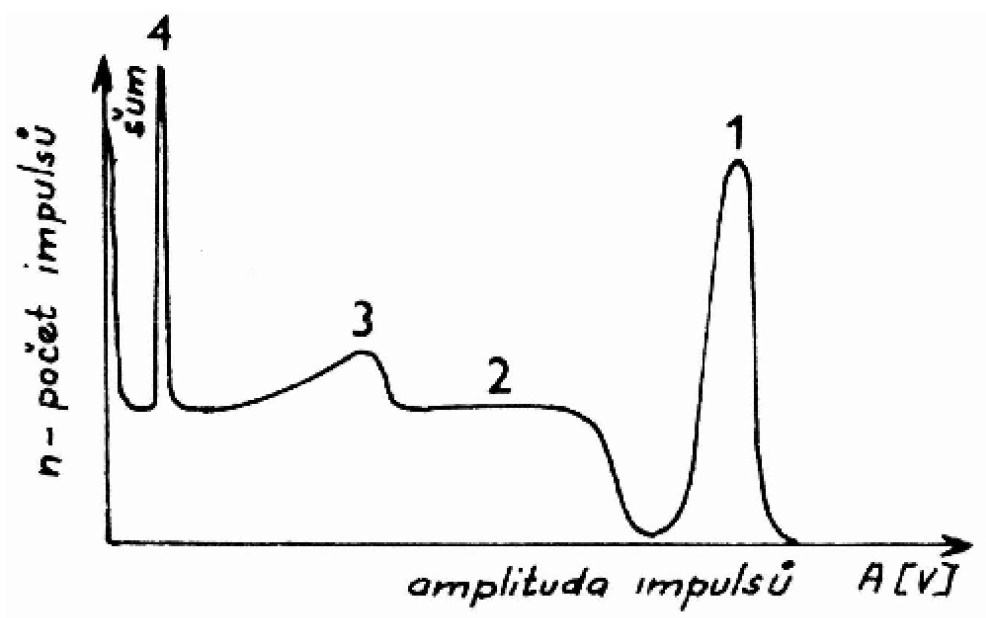
\includegraphics[width=0.6\linewidth]{att/spektrum.jpg}
				    %\vspace*{-1cm}
					\caption{Obrázek typického spektra gama záření. Převzato z \cite{bib:zadani}.}
					\label{fig:s_spektrum}
				\end{center}
				\end{figure}		
			
			\subsubsection{Scintilační detektor}
						Látku, která je schopna reagovat světelnými záblesky (scintilacemi) na pohlcené záření, nazýváme scintilátorem. Takto vytvořené záblesky dále registrujeme pomocí fotonásobiče. Pro náš případ gama záření se dá jako scintilačního prostředí využít monokrystalu NaI(Tl) - tedy jodidu sodného aktivovaného thaliem. Foton přicházející do scintilačního prostředí excituje elektrony z valenční vrstvy do vodivostního pásu a při zpětné deexcitaci se vyzáří nový foton. K tomu ovšem nedojde hned, ale až po nezářivém přechodu fotonu na nižší hladinu. Foton tedy vyzáří až při dalším přechodu a jeho energie je tím pádem nižší, než byla energie fotonu původně přijatého. Takto vyzářený foton již nemůže být pohlcen krystalem. 
						
						V momentu, kdy foton dopadne na fotokatodu, podaří se mu z ní vyrazit několik elektronů. Tyto elektrony následně cestují urychlovány vysokým napětím do násobícího systému na takzvané dynody. Dopadem na dynodu vyrazí každý elektron několik dalších, což vede k zesílení signálu. Po dostatečném zesílení se pak dá zaznamenat standardní elektronikou. 
						
			\subsubsection{Stínění gama záření}
						Když fotony prolétají látkou, jejich energie se nemění, ale následkem srážek se jejich proud postupně zmenšuje. Zeslabení monoenergetického svazku fotonů probíhá podle vztahu
						\begin{equation}
								I(d) = I_0e^{\mu d},
						\label{eq:olovo}
						\end{equation}
						kde $I(d)$ je intenzita svazku s počáteční intenzitou $I_0$ prošlého materiálem o tloušťce $d$. Posledním nedefinovaným symbolem je $\mu$, tedy lineární koeficient útlumu. Pro stínění gama záření se nejčastěji používají materiály s vysokým atomovým číslem, v našem případě olovo. 
			
			\subsubsection{Gaussovo rozdělení}
						K fitování píků využíváme funkci Gauss+konst. s předpisem
						\begin{equation}
								Gauss+konst.(x) = \frac{\alpha}{\sigma \sqrt{2\cdot \pi}} \cdot e^{-\frac{(x-\mu)^2}{2\sigma^2}} + \delta,
						\label{eq:gauss}
						\end{equation}
			kde $\alpha$ je amplituda, $\sigma$ strmost, $\mu$ posunutí a $\delta$ konstanta ve směru $y$.
			
			\subsubsection{Šířka píku v polovině jeho výšky}
						Tato hodnota (jinak zvaná FWHM) se dá spočítat z parametru $\sigma$ Gaussova rozdělení pomocí vzorce
						\begin{equation}
								FWHM = 2 \sqrt{2\ log(2)}\ \sigma.
								\label{eq:fwhm}
						\end{equation}
			
	\subsection{Postup měření}
						Měření spektra jsme prováděli pomocí dvou různých metod. Nejprve manuálním měřením na jednokanálovém analyzátoru a následně měřením na multikanálovém analyzátoru připojeném k počítači. Před samotným měřením jsme aparaturu sestavili následovně:
						\begin{itemize}
								\item Zdroj gama záření jsme umístili na scintilační detektor.
								\item Detektor jsme připojili na zdroj vysokého napětí nastavený na hodnotu 750 V. 
								\item Výstup ze scintilačního detektoru jsme připojili na jednokanálový analyzátor.
								\item (Při druhé metodě na multikanálový analyzátor a ten pak do počítače.)
								\item Z analyzátoru jsme analogový signál přivedli na osciloskop a výstup $\sum$ připojili k čítači.
						\end{itemize}
						Jako první jsme z amplitudy a tloušťky jednotlivých pulsů na osciloskopu na výstupu jednokanálového analyzátoru odhadli a nakreslili tvar spektra pro $^{137}$Cs. Pak jsme pokračovali měřením jednokanálovým analyzátorem a postupovali podle následujícího postupu:
						\begin{enumerate}
								 \item Zapneme zdroj vysokého napětí, jednokanálový analyzátor a čítač impulsů.
								 \item Přepneme jednokanálový analyzátor do manuálního módu.
								 \item Nastavíme dolní diskriminační hladinu pomocí kolečka BASE a přepínáním tlačítka WINDOW také šířku okna na 100 mV. 
								 \item Zaznamenáváme hodnoty z čítače při zvyšování diskriminační hladiny do té doby, než nezačneme dostávat na čítači konzistentně hodnoty blízké nule, nebo nedosáhneme hladiny 10 V.
						\end{enumerate}
						Měření mnohokanálovým analyzátorem se nám bohužel nepodařilo uskutečnit z důvodu technických problémů. Data, která jsme měli naměřit, jsme tedy obdrželi přímo od asistentů v praktiku a dále pracovali s nimi. 
				
	\subsection{Naměřené hodnoty}
					Spektrum $^{137}$Cs pozorované osciloskopem je přiloženo k protokolu. To samé spektrum naměřené jednokanálovým analyzátorem pomocí manuálního měření je vidět na Obr. \ref{fig:g_Cs_jedno}. Spektra přiložených zářičů ($^{137}$Cs, $^{60}$Co, $^{241}$Am a $^{133}$Ba) naměřená mnohokanálovým analyzátorem jsou vyneseny v grafech na Obr. \ref{fig:g_Cs_vice}, \ref{fig:g_Co_vice}, \ref{fig:g_Am_vice} a \ref{fig:g_Ba_vice} i s určenými výraznými píky. V naměřeném spektru $^{137}$Cs (Obr. \ref{fig:g_Cs_vice}) jsou pak určeny i hodnoty dalších jevů. Pomocí zářičů $^{137}$Cs a $^{60}$Co určená kalibrační křivka je vykreslena na Obr. \ref{fig:g_kalib} a ze všech naměřených spekter zjištěná závislost rozlišení spektrometru na energii gama záření v grafu na Obr. \ref{fig:g_rozliseni}. Spektrum neznámého zářiče je k vidění na Obr. \ref{fig:g_Un_vice} i s vyznačenými píky (anihilační a úplného pohlcení). Spektrum pozadí v místnosti je na Obr. \ref{fig:g_pozadi_vice} a grafické určení závislosti koeficientu útlumu olova na energii gama záření na Obr. \ref{fig:g_BaCoCsPb} se spektrem (pro ilustraci) na Obr. \ref{fig:g_BaCoCsPb2}.
					
					Z dat  mnohokanálového analyzátoru jsme určili píky úplného pohlcení pro jednotlivé zářiče (pomocí fitu funkcí Gauss+konst. (\ref{eq:gauss})) následovně:
					\begin{center}
					\begin{tabular}{rrrr}
							\textbf{Zářič} & \multicolumn{1}{c}{\textbf{Naše hodnoty}} & \multicolumn{1}{c}{\textbf{Tabulkové hodnoty \cite{bib:net}}}\\
					        $^{137}$Cs & $(663,3 \pm 0,4)$ keV &  $661,657$ keV \\
					        $^{60}$Co & $(1171,6 \pm 0,7)$ keV &  $1173,237$ keV  \\
					                             & $(1319,1 \pm 0,6)$ keV & $1332,501$ keV\\
					        $^{241}$Am & $(64,2 \pm 0,2)$ keV & $59,541$ keV\\					        
					        $^{133}$Ba & $(89,8 \pm 0,2)$ keV & $80,997$ keV \\
					                              & $(382,6 \pm 0,4)$ keV & $356,017$ keV\\
					\end{tabular}
					\end{center}
					\vspace{0.4cm}
					
					V naměřeném spektru $^{137}$Cs jsme dále pozorovali následující jevy na odpovídajících energiích (\ref{eq:gauss})  (žádný další pík, který by se dal označit za součtový jsem v grafu spektra nevypozoroval):
					\begin{center}
					\begin{tabular}{rr}
							\multicolumn{1}{c}{\textbf{Druh jevu} } & \multicolumn{1}{c}{\textbf{Energie} }\\
							pík zpětného rozptylu & $(202 \pm 2)$ keV \\
							Comptonova hrana & $(470 \pm 5)$ keV \\
							rentgenový pík & $(22,2 \pm 0,6)$ keV \\
					\end{tabular}
					\end{center}
					\vspace{0.4cm}
					
					Neznámý zářič vychází dle tabulek nejblíže zářiči $^{22}$Na. 
					\begin{center}
					\begin{tabular}{rrr}
							\multicolumn{1}{c}{\textbf{Druh jevu} } & \multicolumn{1}{c}{\textbf{Naše hodnoty}} & \multicolumn{1}{c}{\textbf{Tabulkové hodnoty \cite{bib:net}}}\\
					        elektron-pozitronová anihilace &  $(539,3 \pm 0,2)$ keV & $511$ keV\\
					        pík úplného pohlcení & $(1277 \pm 1)$ keV & $1274,53$ keV\\
					\end{tabular}					
					\end{center}
					
					Parametr kalibrační křivky ve tvaru $f(N)=a\cdot N$ (kde $N$ je číslo kanálu) jsme z dat určili jako 
					\begin{equation}
							a = (0,658 \pm 0,003)\ \unit{keV}.
					\end{equation}
					
					Závislost rozlišení spektrometru na energii jsme určili lineárním proložením jako 
					\begin{equation}
							\Delta E(E) = (0,04 \pm 0,01)  E + (31 \pm 9).
					\end{equation}
					
					Závislost koeficientu útlumu olova na energii gama záření jsme (z dat zářičů $^{137}$Cs, $^{60}$Co a $^{133}$Ba současně za použití (\ref{eq:olovo})) určili jako exponenciální ve tvaru
					\begin{equation}
							\mu(E) = \frac{1}{aE}, \qquad a=(7 \pm 1) \cdot 10^{-5}.
					\end{equation}
							
	\subsection{Diskuse}
					Pozorování spektra $^{137}$Cs na výstupu z jednokanálového analyzátoru se nám podařilo, ale je třeba podotknout, že nákres je pouze velmi nepřesný odhad a rozhodně by se na něj nedalo spolehnout. Jednotlivé pulsy se na displeji osciloskopu měnily příliš rychle a zhruba stejně často zasahovaly na místa ve velkých intervalech. Při této metodě také nemůžeme rozumně určit rozsah grafu (jednotky jsou tedy na nákresu uvedeny jen pro rozměr). 
					
					Při měření spektra impulsů $^{137}$Cs jednokanálovým analyzátorem pomocí manuálního měření jsme neměřili až do 10 V, jelikož už od poloviny tohoto rozsahu byly hodnoty takřka nulové. Na čítači jsme nastavili průměrování počtu impulsů na dobu 10 s pro konzistentnější hodnoty, i tak ale v některých případech na stejném rozsahu napětí osciloval tento počet v řádu desítek procent hodnoty. Měření by šlo zpřesnit průměrováním na čítači za ještě delší čas nebo volbou menšího okna (pokud by to přístroj dovoloval). Výsledky z této metody opticky odpovídají dodaným výsledkům z multikanálu a měření se tak dá považovat za úspěšné. 
					
					Všechna měření obsahující multikanálový analyzátor jsme z důvodu technických problémů nemohli provést a pracovali jsme tak s dříve a někým jiným naměřenými daty. Při většině pokusů o měření se počítač rozhodl (možná z důvodu probíjejícího detektoru) interpretovat signál z analyzátoru jako pokyny pro kurzor myši a v závislosti na přiloženém zářiči jím rychleji či pomaleji pohyboval a zuřivě klikal (ověřeno pro $^{137}$Cs a $^{60}$Co). Poté co několikrát přesunul ikony na ploše na jiná místa, lištu Startu na levou či pravou hranu obrazovky, případně opakovaně zavřel předem otevřený program MEASURE, rozhodli jsme se snažení ukončit. Ze strany jednoho z devíti pozorujících asistentů padl návrh zaznamenávat tímto stylem spektrum v programu Malování a dívat se kolik toho detektor nakreslí za konkrétní časový úsek. Tuto metodu jsme již však neměli možnost vyzkoušet. 
					
					Jednotlivá dodaná spektra přiložených zářičů jsme tedy analyzovali a určili u nich výrazné píky (po kalibraci). Tyto jsme srovnali s tabulkovými hodnotami a ač neleží přímo v chybových intervalech určených fitem (\ref{eq:gauss}), stále velmi dobře odpovídají. 
					
					Kalibrační křivku se nám podařilo určit s relativně dobrou přesností i jen ze tří píků zmíněných zářičů a jejich tabulkových \cite{bib:net} hodnot. Přesnější by bylo použití lineární závislosti ve tvaru $f(x) = ax+b$, ale ta by umožňovala v hodnotách $x$ blízkých nule záporné hodnoty energií a nebyla by tedy fyzikálně reálná. 
					
					Závislost rozlišení spektrometru na energii se nám určit podařilo, nicméně lineární proložení se v tomto případě jeví jako relativně nepřesné, vzhledem k tomu do jak málo chybových intervalů (chyby byly počítány z fitu jednotlivých píků) přímka zasahuje. Možné je opět, že závislost není lineární, případně že se do rozmístění píků propaguje nepřesnost kalibrace.
					
					Jevy ve spektru $^{137}$Cs se nám podařilo určit dobře, až na pozici Comptonovy hrany, která se nedá rozumně získat proložením a bylo ji tak třeba z dat pouze nepřesně odhadnout. Součtový pík jsme ve spektru nepozorovali. 
					
					Neznámý zářič jsme úspěšně určili jako $^{22}$Na. Ve spektru jsem nebyl schopen jednoznačně určit žádné další výrazné jevy - možný je výskyt detekce dvou anihilačních fotonů a tedy píku kolem hodnoty 1022 keV. Pík ale na jasný závěr není dostatečně znatelný.
					
					Ve spektru pozadí se mi nepodařilo určit jednoznačně žádné přirozené zářiče. Tabulkově \cite{bib:net} do daného rozsahu energií patří nejrůznější zářiče a pík je na přesnější určení příliš široký. Při odečítání pozadí v některých případech (např. více zářičů současně) vycházely počty výskytů výrazně (např. -100) v záporných hodnotách. Proto jsem při zpracovávání jiných spekter než jednotlivých zářičů pozadí neodečítal, což mohlo ztížit hledání píků v oblasti $0-450$ keV. Pozice výrazných píků a píků ve zbytku spektra to však nemohlo výrazně ovlivnit.  
					
					Závislost koeficientu útlumu olova na energii gama záření se nám podařilo určit relativně dobře a odpovídá porovnání obou spekter, kde docházelo očividně k největšímu útlumu při malých energiích. Opět vyvstává otázka, jestli je závislost opravdu exponenciální, jelikož tlumení záření s velmi nízkou energií nejspíš nebude nekonečné. Rozdíl dat se naopak při energiích větších než zhruba $500$ keV dostával v polovině případů do záporu, což by mohlo být způsobeno nízkou rozlišovací schopností detektoru u vysokých energií a inkonzistencí hodnot na tomto rozsahu (a jejich následnému odečítání). Navíc neznáme tloušťku olověné destičky, se kterou bylo při měření stíněno, takže jsem pro účely fitu předpokládal tloušťku $1,5$ mm. I kdyby ale byla tloušťka jiná, pozorovaný trend se nezmění.
			
\section{Závěr}
		Osciloskopem jsme pozorovali spektrum $^{137}$Cs na výstupu z jednokanálového analyzátoru a načrtli jsme tvar spektra, který jsme přiložili k protokolu. Úspěšně jsme naměřili spektrum impulsů $^{137}$Cs jednokanálovým analyzátorem pomocí manuálního měření a spektrum jsme graficky zpracovali. Mnohokanálovým analyzátorem se nám měření z technických důvodů (viz Diskuse) nepodařilo provést a všechny následující úlohy jsme tedy prováděli až od analýzy dat. Určili jsme výrazné píky přiložených zářičů a porovnali je s tabulkovými hodnotami. Z dat naměřených pro dva z nich jsme určili kalibrační křivku a použili ji při zpracovávání všech spekter naměřených mnohokanálovým analyzátorem. S využitím všech naměřených spekter jsme určili závislost rozlišení spektrometru na energii gama záření. Z naměřeného spektra $^{137}$Cs jsme úspěšně určili hodnotu tří jevů. Dále jsme z dat určili neznámý zářič a při analýze využili naměřené pozadí v místnosti. Nakonec se nám podařilo graficky určit závislost koeficientu útlumu olova na energii gama záření, byť za pouhého odhadu tloušťky stínící vrstvy. 
		
\section {Použitá literatura}
% --- Literatura a reference -------------------------------------------
\begingroup
\renewcommand{\section}[2]{}

\begin{thebibliography}{9}
\bibitem{bib:zadani} Kolektiv KF, \emph{Návod k úloze: Měření spektra gama záření scintilačním počítačem} [Online], [cit. \today] \newline 
http://praktikum.fjfi.cvut.cz/pluginfile.php/420/mod\_resource/content/7/gamma\_navod\_JF\_v2.pdf

\bibitem{bib:net} LUNDS Universitet, \emph{LBNL Isotopes Project} [Online], [cit. \today] \newline http://ie.lbl.gov/toi/index.asp

%\bibitem{bib:h3} Petr Chaloupka, \emph{Jak zpracovávat data} [Online], [cit. \today] \newline  https://dl.dropboxusercontent.com/u/11296940/zfm/h3.pdf

%\bibitem{bib:navody} Kolektiv KF, \emph{Návody k přístrojům} [Online], [cit. \today] \newline http://praktikum.fjfi.cvut.cz/documents/chybynav/navody-o.pdf

%\bibitem{bib:chyby} Kolektiv KF, \emph{Chyby měření} [Online], [cit. \today] \newline http://praktikum.fjfi.cvut.cz/documents/chybynav/chyby-o.pdf

%\bibitem{bib:ctverce} Kolektiv KACH UPOL, \emph{Hodnocení analytických výsledků} [Online], [cit. \today] \newline http://ach.upol.cz/ucebnice/hodnoceni7.htm

%\bibitem{bib:tlak} Český hydrometeorologický ústav, \emph{Meteogramy Aladin} [Online], [cit. \today]  \newline http://bit.ly/AladinMeteogramy

%\bibitem{bib:tabulky} J. Mikulčák a kol., Matematické, fyzikální a chemické tabulky \& vzorce. Prometheus,
%Praha 2009.\newline
%ISBN 978-80-7196-264-9

%\bibitem{bib:repo} Kolektiv autorů, \emph{Repozitář zdrojů k praktiku} [Online], [cit. \today] \newline  http://github.com/roesel/praktika

\end{thebibliography}
\endgroup
% ----------------------------------------------------------------------
\setcounter{equation}{0}
\numberwithin{equation}{section}
\clearpage
\part{Přílohy}

\section{Domácí příprava}
	Domácí příprava je přiložena k protokolu.
%\clearpage
%\subsection{Statistické zpracování dat}
%	Pro statistické zpracování využíváme aritmetického průměru:
%	\begin{equation} \label{eq:aritmeticky_prumer}
%	\overline{x} = \frac{1}{n}\sum\limits_{i=1}^{n}x_i,
%	\end{equation}
%	
%	jehož chybu spočítáme jako 
%	\begin{equation} \label{eq:chyba_aritmetickeho_prumeru}
%	\sigma_0 = \sqrt{\frac{1}{n(n-1)} \sum\limits_{i=1}^{n}\left( x_i - \overline{x} \right)^2 },
%	\end{equation}
%	
%	kde $ x_i $ jsou jednotlivé naměřené hodnoty, $ n $ je počet měření, $ \overline{x} $ aritmetický průměr a $ \sigma_0 $ jeho chyba \cite{bib:chyby}.
%	
%Při nepřímém měření počítáme hodnotu s chybou dle následujících vztahů:
%	\begin{equation}
%	u = f(x, y, z, \ldots),
%	\end{equation}
%	\begin{displaymath}
%	x = (\overline{x} \pm \sigma_x), \qquad
%	y = (\overline{y} \pm \sigma_y), \qquad
%	z = (\overline{z} \pm \sigma_z), \qquad
%	\ldots,
%	\end{displaymath}
%	
%	kde $ u $ je veličina, kterou určujeme nepřímo z měřených veličin $ x, y, z, \ldots $ 
%	
%	Pak
%	\begin{displaymath}
%	\overline{u} = f(\overline{x}, \overline{y}, \overline{z}, \ldots),
%	\end{displaymath}
%	\begin{equation}\label{eq:chyba_neprime_mereni}
%	\sigma_u = \sqrt{\left( \frac{\partial f}{\partial x} \right)^2 \sigma^2_x + \left( \frac{\partial f}{\partial y} \right)^2 \sigma^2_y + \left( \frac{\partial f}{\partial z} \right)^2 \sigma^2_z + \ldots},
%	\end{equation}
%	\begin{displaymath}
%	u = (\overline{u} \pm \sigma_ u).
%	\end{displaymath}
%%	
%V případě, že máme několik různě přesných měření stejné veličiny, používáme vztah pro vážený průměr:
%	\begin{equation} 
%	\bar{x}=\frac{\sum\limits_{i=1}^{n}p_{i}x_{i}}{\sum\limits_{i=1}^{n}p_{i}},
%	\end{equation}
%	
%	kde $\bar{x}$ je vážený průměr, $x_{i}$ jsou jednotlivá měření a pro $p_{i}$ platí
%	 
%	\begin{equation}
%	p_{i}=\frac{1}{\sigma_{i}^{2}},
%	\end{equation}
%	
%	kde $\sigma_{i}$ jsou jednotlivé chyby daných měření.
%	 
%	Celkovou chybu tedy vypočítáme ze vztahu
%	\begin{equation} \label{eq:vazeny_prumer}
%	\sigma_{0}=\sqrt{\frac{1}{\sum\limits_{i=1}^{n}p_{i}}}.
%	\end{equation}
%
%\subsubsection{Metoda nejmenších čtverců}
%Snažíme-li se metodou nejmenších čtverců proložit data lineární závislostí $Y_i = ax_i+b$, dosazujeme hodnoty $x_i, y_i$ a snažíme se najít parametry $a$ a $b$ tak, aby byl součet všech kvadratických odchylek $\Delta Y_i^2$ minimální. Toho dosáhneme pomocí následujících vzorců \cite{bib:ctverce} :
%\begin{equation}\label{eq:ctverce_a}
%		a = \frac{n\sum\limits_{i=1}^{n}{x_i y_i}  - \sum\limits_{i=1}^{n}{x_i}\sum\limits_{i=1}^{n}{y_i}}{n\sum\limits_{i=1}^{n}{x_i^2}  - \left(\sum\limits_{i=1}^{n}{x_i}\right)^2}, \qquad \qquad
%		\sigma_a = \sqrt{\frac{n\sum\limits_{i=1}^{n}{(y_i - Y_i)^2} }{(n-2)\left(\sum\limits_{i=1}^{n}{x_i^2}  - \left(\sum\limits_{i=1}^{n}{x_i}\right)^2\right)}},
%\end{equation}
%
%\begin{equation}\label{eq:ctverce_b}
%		b = \frac{\sum\limits_{i=1}^{n}{x_i^2} \sum\limits_{i=1}^{n}{y_i}  - \sum\limits_{i=1}^{n}{x_i}\sum\limits_{i=1}^{n}{x_i y_i}}{n\sum\limits_{i=1}^{n}{x_i^2}  - \left(\sum\limits_{i=1}^{n}{x_i}\right)^2}, \qquad \qquad
%		\sigma_b = \sqrt{\frac{\sum\limits_{i=1}^{n}{x_i^2}\sum\limits_{i=1}^{n}{(y_i - Y_i)^2} }{n(n-2)\left(\sum\limits_{i=1}^{n}{x_i^2}  - \left(\sum\limits_{i=1}^{n}{x_i}\right)^2\right)}}.
%\end{equation}
	
%\clearpage
\subsection{Tabulky a grafy}

	\begin{figure}[h!]
	\begin{center}
	    \vspace*{-1cm}
		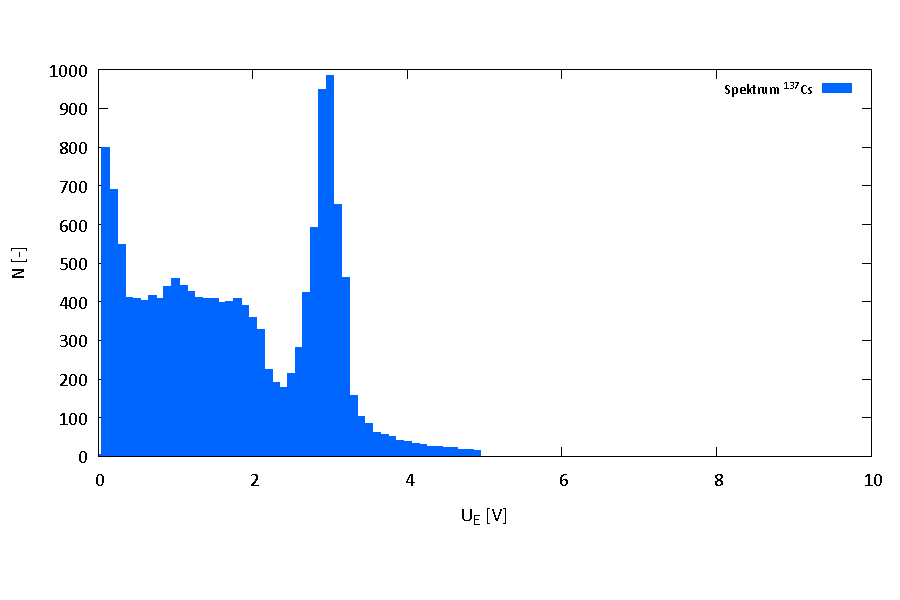
\includegraphics[width=\linewidth]{../gnuplot/Cs1.pdf}
	    \vspace*{-2cm}
		\caption{Spektrum $^{137}$Cs naměřené jednokanálovým analyzátorem pomocí manuálního měření - $U_E$ je napětí odpovídající energii pohlceného záření, $N$ počet pulsů zaznamenaný čítačem.}
		\label{fig:g_Cs_jedno}
	\end{center}
	\end{figure}	
	
	\begin{figure}[h!]
	\begin{center}
	    \vspace*{-1cm}
		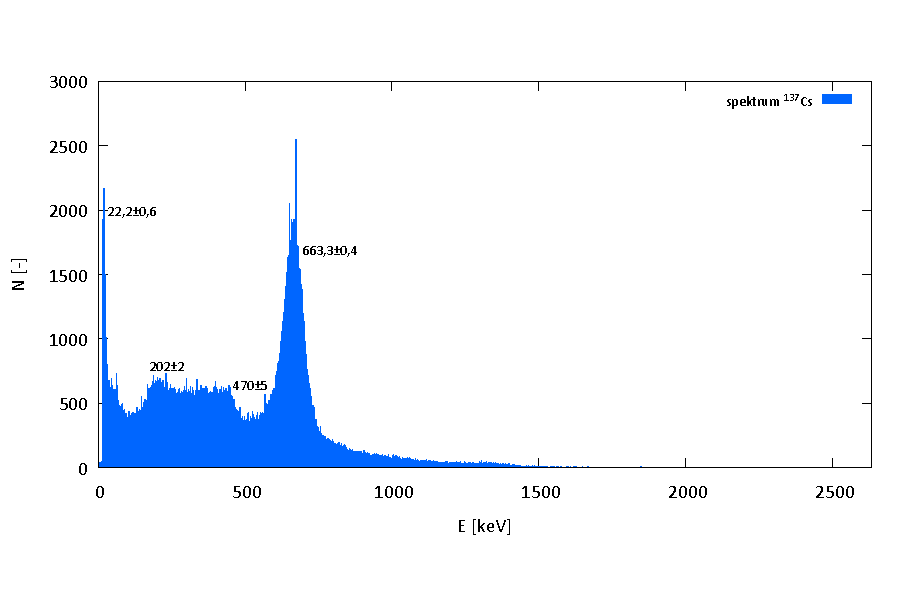
\includegraphics[width=\linewidth]{../gnuplot/solo/Cs.pdf}
	    \vspace*{-2cm}
		\caption{Spektrum $^{137}$Cs naměřené vícekanálovým analyzátorem - $E$ je energie, $N$ počet pulsů zaznamenaný počítačem. Do grafu jsou vyneseny hodnoty energií (určené fitem Gauss+konst. (\ref{eq:gauss})) pro rentgenový pík, pík zpětného rozptylu, Comptonovu hranu a fotopík.}
		\label{fig:g_Cs_vice}
	\end{center}
	\end{figure}	
	
	\begin{figure}[h!]
	\begin{center}
	    \vspace*{-1cm}
		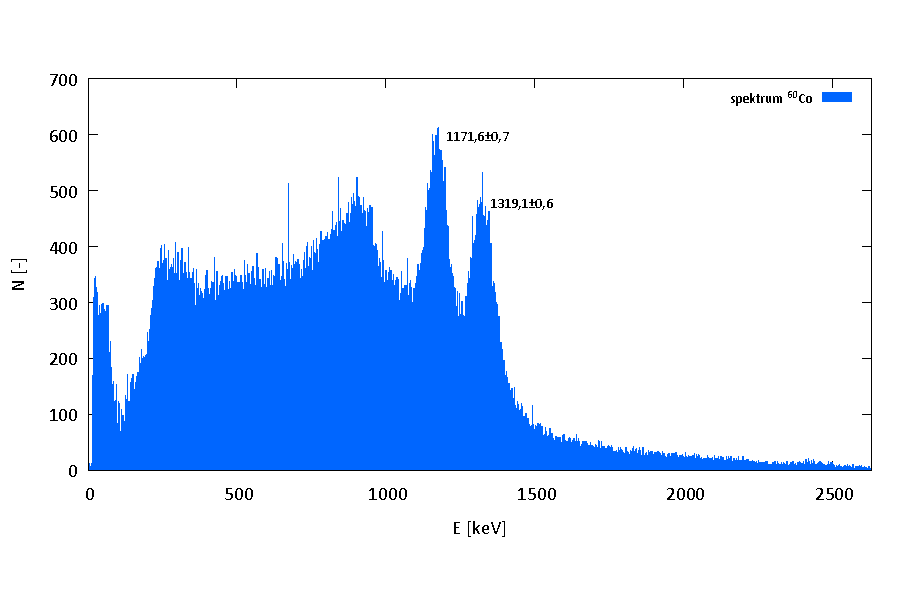
\includegraphics[width=\linewidth]{../gnuplot/solo/Co.pdf}
	    \vspace*{-2cm}
		\caption{Spektrum $^{60}$Co naměřené vícekanálovým analyzátorem - $E$ je energie, $N$ počet pulsů zaznamenaný počítačem. Do grafu jsou vyneseny hodnoty energií (určené fitem Gauss+konst. (\ref{eq:gauss})) pro píky úplného pohlcení.}
		\label{fig:g_Co_vice}
	\end{center}
	\end{figure}	
	
	\begin{figure}[h!]
	\begin{center}
	    \vspace*{-1cm}
		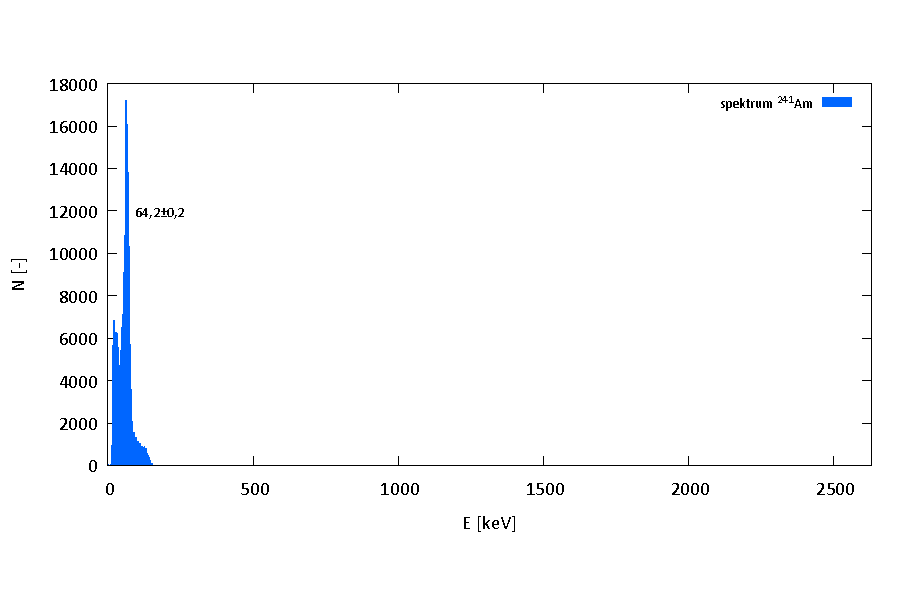
\includegraphics[width=\linewidth]{../gnuplot/solo/Am.pdf}
	    \vspace*{-2cm}
		\caption{Spektrum $^{241}$Am naměřené vícekanálovým analyzátorem - $E$ je energie, $N$ počet pulsů zaznamenaný počítačem. Do grafu je vynesena hodnota energie (určené fitem Gauss+konst. (\ref{eq:gauss})) pro pík úplného pohlcení.}
		\label{fig:g_Am_vice}
	\end{center}
	\end{figure}	
	
	\begin{figure}[h!]
	\begin{center}
	    \vspace*{-1cm}
		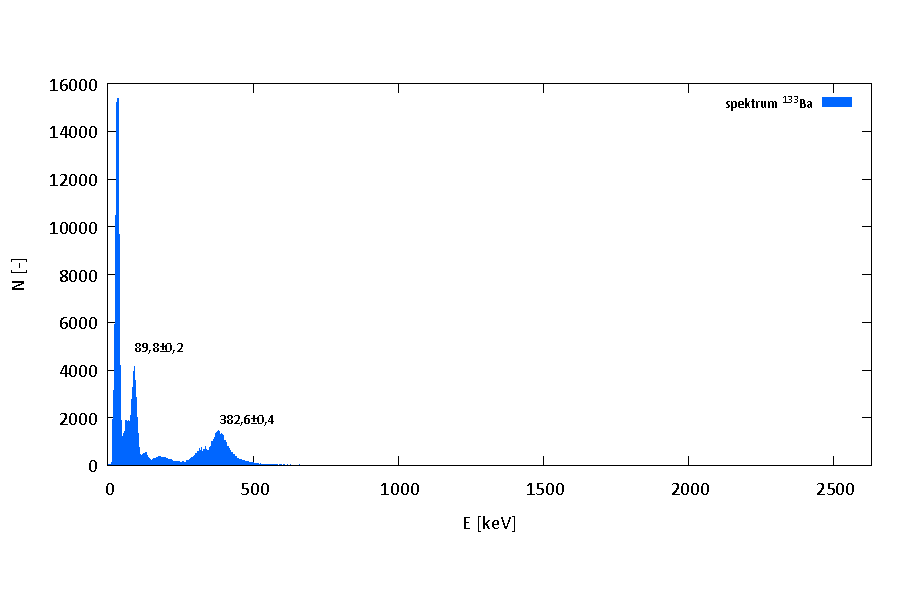
\includegraphics[width=\linewidth]{../gnuplot/solo/Ba.pdf}
	    \vspace*{-2cm}
		\caption{Spektrum $^{133}$Ba naměřené vícekanálovým analyzátorem - $E$ je energie, $N$ počet pulsů zaznamenaný počítačem. Do grafu jsou vyneseny hodnoty energií (určené fitem Gauss+konst. (\ref{eq:gauss})) pro píky úplného pohlcení.}
		\label{fig:g_Ba_vice}
	\end{center}
	\end{figure}	
	
	\begin{figure}[h!]
	\begin{center}
	    \vspace*{-1cm}
		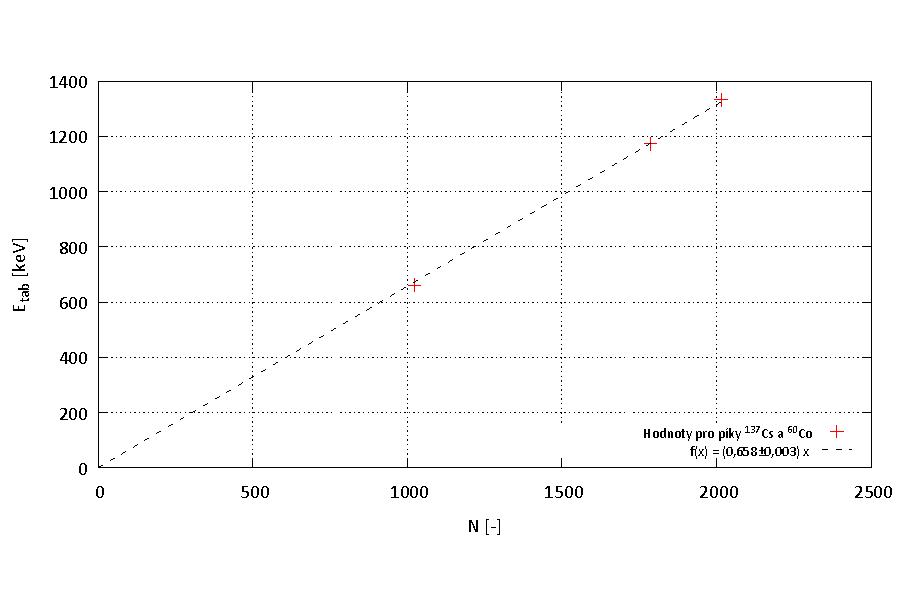
\includegraphics[width=\linewidth]{../gnuplot/kalib.pdf}
	    \vspace*{-2cm}
		\caption{Kalibrační křivka ve tvaru $E(N) = a\cdot N$, kde $N$ je číslo kanálu a $E_{tab}$ jemu odpovídající energie \cite{bib:net}.}
		\label{fig:g_kalib}
	\end{center}
	\end{figure}	
	
	\begin{figure}[h!]
	\begin{center}
	    \vspace*{-1cm}
		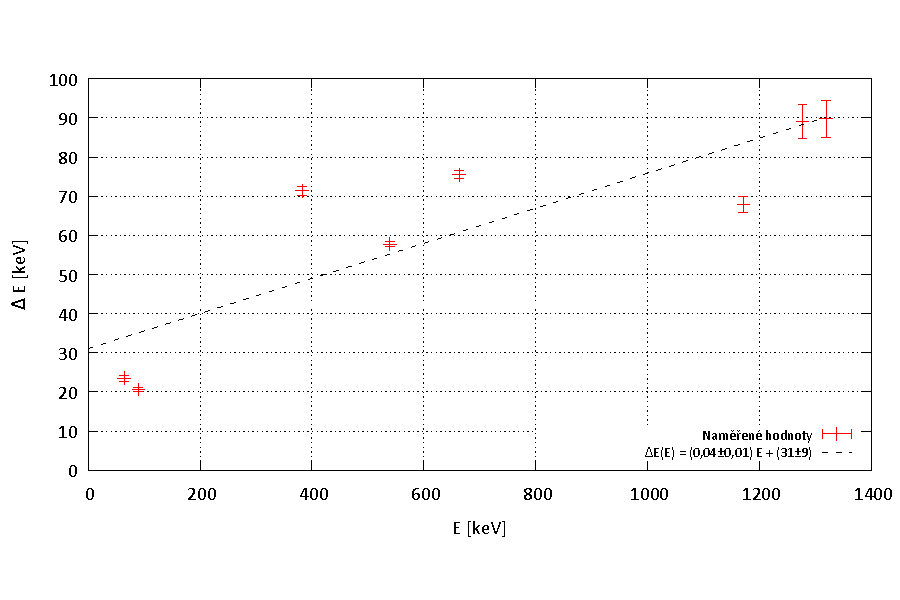
\includegraphics[width=\linewidth]{../gnuplot/rozliseni.pdf}
	    \vspace*{-2cm}
		\caption{Závislost rozlišení spektrometru na energii gama záření s využitím všech naměřených spekter. $\Delta E$ je šířka píku úplného pohlcení spočítaná podle (\ref{eq:fwhm}) a $E$ energie píku daného prvku. }
		\label{fig:g_rozliseni}
	\end{center}
	\end{figure}						

	\begin{figure}[h!]
	\begin{center}
	    \vspace*{-1cm}
		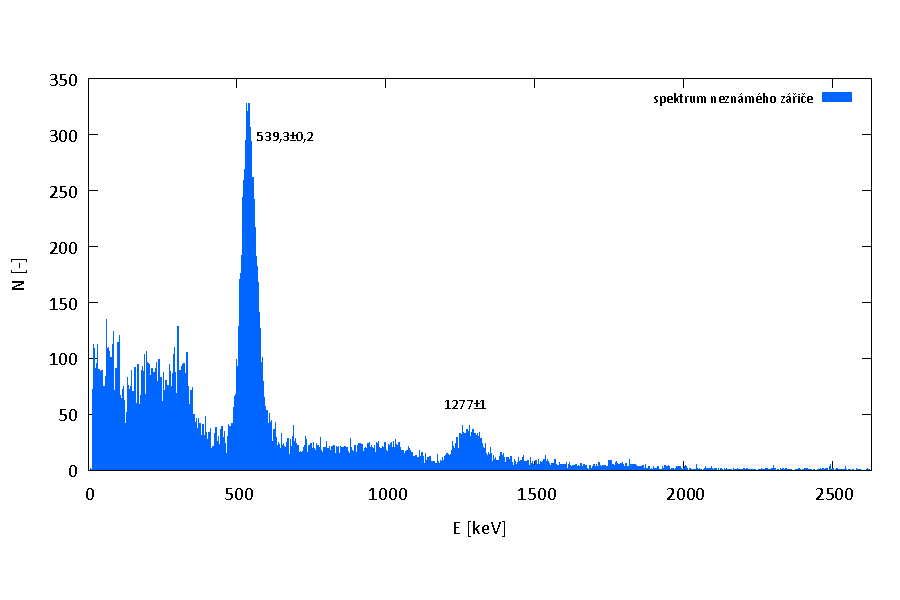
\includegraphics[width=\linewidth]{../gnuplot/solo/Un.pdf}
	    \vspace*{-2cm}
		\caption{Spektrum neznámého zářiče naměřené vícekanálovým analyzátorem - $E$ je energie, $N$ počet pulsů zaznamenaný počítačem. Do grafu jsou vyneseny hodnoty energií (určené fitem Gauss+konst. (\ref{eq:gauss})) pro další význačné píky (anihilační a úplného pohlcení).}
		\label{fig:g_Un_vice}
	\end{center}
	\end{figure}
	
	\begin{figure}[h!]
	\begin{center}
	    \vspace*{-1cm}
		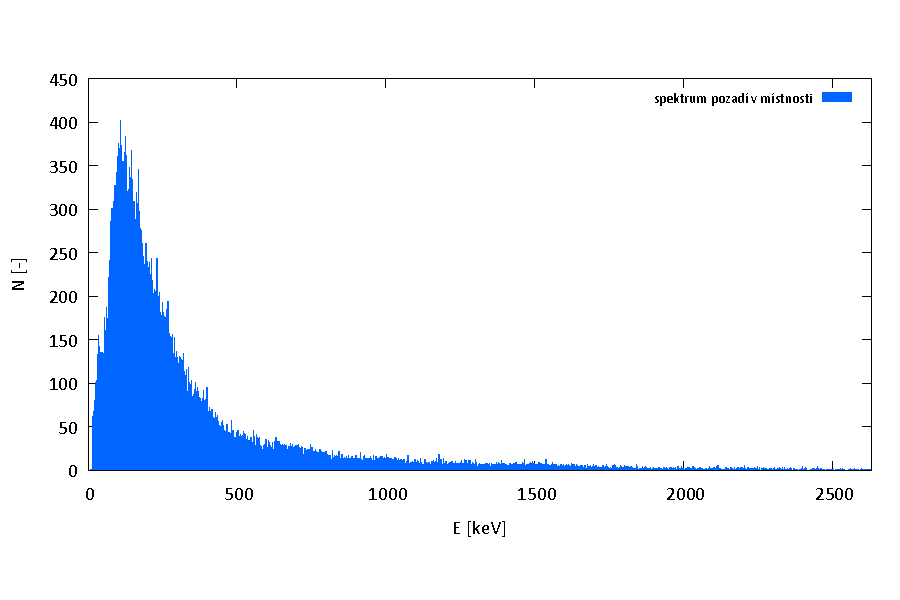
\includegraphics[width=\linewidth]{../gnuplot/solo/background.pdf}
	    \vspace*{-2cm}
		\caption{Spektrum pozadí v místnosti naměřené vícekanálovým analyzátorem - $E$ je energie, $N$ počet pulsů zaznamenaný počítačem.}
		\label{fig:g_pozadi_vice}
	\end{center}
	\end{figure}	

	\begin{figure}[h!]
	\begin{center}
	    \vspace*{-1cm}
		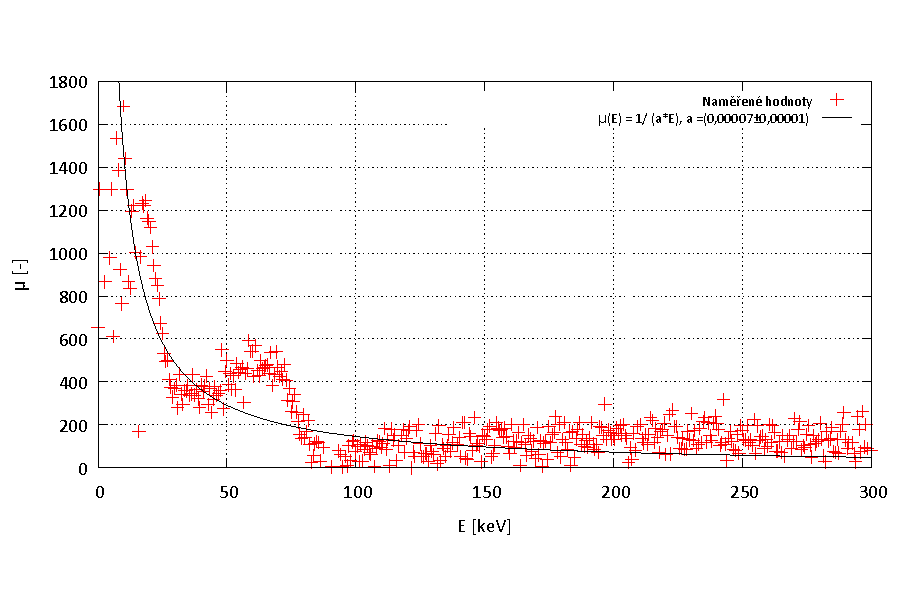
\includegraphics[width=\linewidth]{../gnuplot/BaCoCsandPb.pdf}
	    \vspace*{-2cm}
		\caption{Závislost koeficientu útlumu $\mu$ olova na energii gama záření $E$ (z měření $^{137}$Cs, $^{60}$Co a $^{133}$Ba současně vícekanálovým analyzátorem).}
		\label{fig:g_BaCoCsPb}
	\end{center}
	\end{figure}	
	
	\begin{figure}[h!]
	\begin{center}
	    \vspace*{-1cm}
		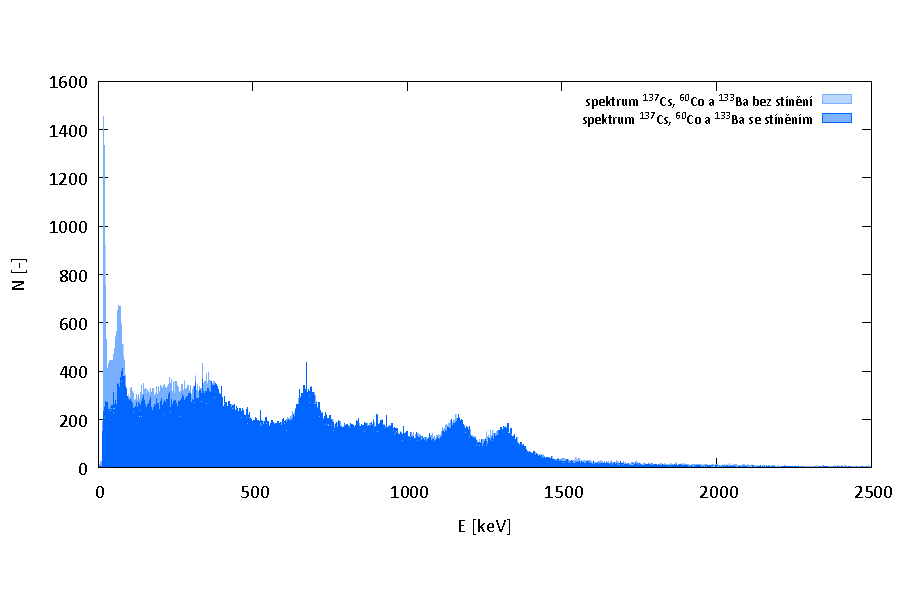
\includegraphics[width=\linewidth]{../gnuplot/BaCoCsandPb2.pdf}
	    \vspace*{-2cm}
		\caption{Spektrum $^{137}$Cs, $^{60}$Co a $^{133}$Ba naměřené vícekanálovým analyzátorem - $E$ je energie, $N$ počet pulsů zaznamenaný počítačem. Světlejší je spektrum zářičů bez stínění, tmavší pak to měřené po přidání olověné destičky.}
		\label{fig:g_BaCoCsPb2}
	\end{center}
	\end{figure}	
	
	

%
%\clearpage
%\subsection{Schémata}
%
%\clearpage
	
% --- Konec dokumentu --------------------------------------------------


\end{document}

